\chapter{PoC}%
\label{ch:PoC}

% TODO: Trek een duidelijke conclusie, in de vorm van een antwoord op de
% onderzoeksvra(a)g(en). Wat was jouw bijdrage aan het onderzoeksdomein en
% hoe biedt dit meerwaarde aan het vakgebied/doelgroep? 
% Reflecteer kritisch over het resultaat. In Engelse teksten wordt deze sectie
% ``Discussion'' genoemd. Had je deze uitkomst verwacht? Zijn er zaken die nog
% niet duidelijk zijn?
% Heeft het onderzoek geleid tot nieuwe vragen die uitnodigen tot verder 
%onderzoek?

\section{Inleiding}
Deze sectie beschrijft de implementatie van het systeem, waarbij wordt ingegaan op de ontwikkeling van de individuele componenten, de integratie van de componenten, en de uiteindelijke inzet van de applicatie. De focus ligt op de technische realisatie van de architectuur zoals beschreven in Hoofdstuk 3.


\section{Android Applicatie}
De Android-applicatie \autocite{VisionAndroid} is essentieel voor de interactie met eindgebruikers en is specifiek ontworpen om efficiënt gebruik te maken van de functionaliteiten die moderne smartphones bieden. Het ontwikkelingsproces omvatte verschillende belangrijke aspecten die hieronder in detail worden beschreven:

\begin{itemize}
    \item \textbf{Gebruikersinterface:} De interface is ontwikkeld met een focus op gebruikersvriendelijkheid. De gebruikersinterface maakt gebruik van een modern ontwerp dat responsive is over verschillende schermgroottes en -resoluties. Belangrijke UI-elementen omvatten een interactieve camera-interface, een galerijweergave van recente opnames, en een dynamisch informatiepaneel dat updates ontvangt van de backend.
    
    \item \textbf{Camera-functionaliteit:} De camera-integratie maakt gebruik van de Android Camera2 API, die uitgebreide controle biedt over camerafuncties zoals belichting, focus en resolutie. Dit stelt gebruikers in staat om hoogwaardige afbeeldingen te maken die geschikt zijn voor verder analyse. De app bevat ook functionaliteit om foto's in real-time te beoordelen en te bewerken voordat ze worden verzonden.
    
    \item \textbf{Netwerkcommunicatie:} Om de afbeeldingen te verzenden naar de backend voor verwerking, implementeert de applicatie robuuste netwerkcommunicatiemechanismen. Dit omvat het gebruik van Retrofit voor gestroomlijnde HTTP-verzoeken en responsverwerking. Secure Socket Layer (SSL) encryptie wordt gebruikt om de veiligheid van dataoverdracht te garanderen.
    
\end{itemize}



\subsection{User interface}

\begin{figure}[h!]
    \centering
    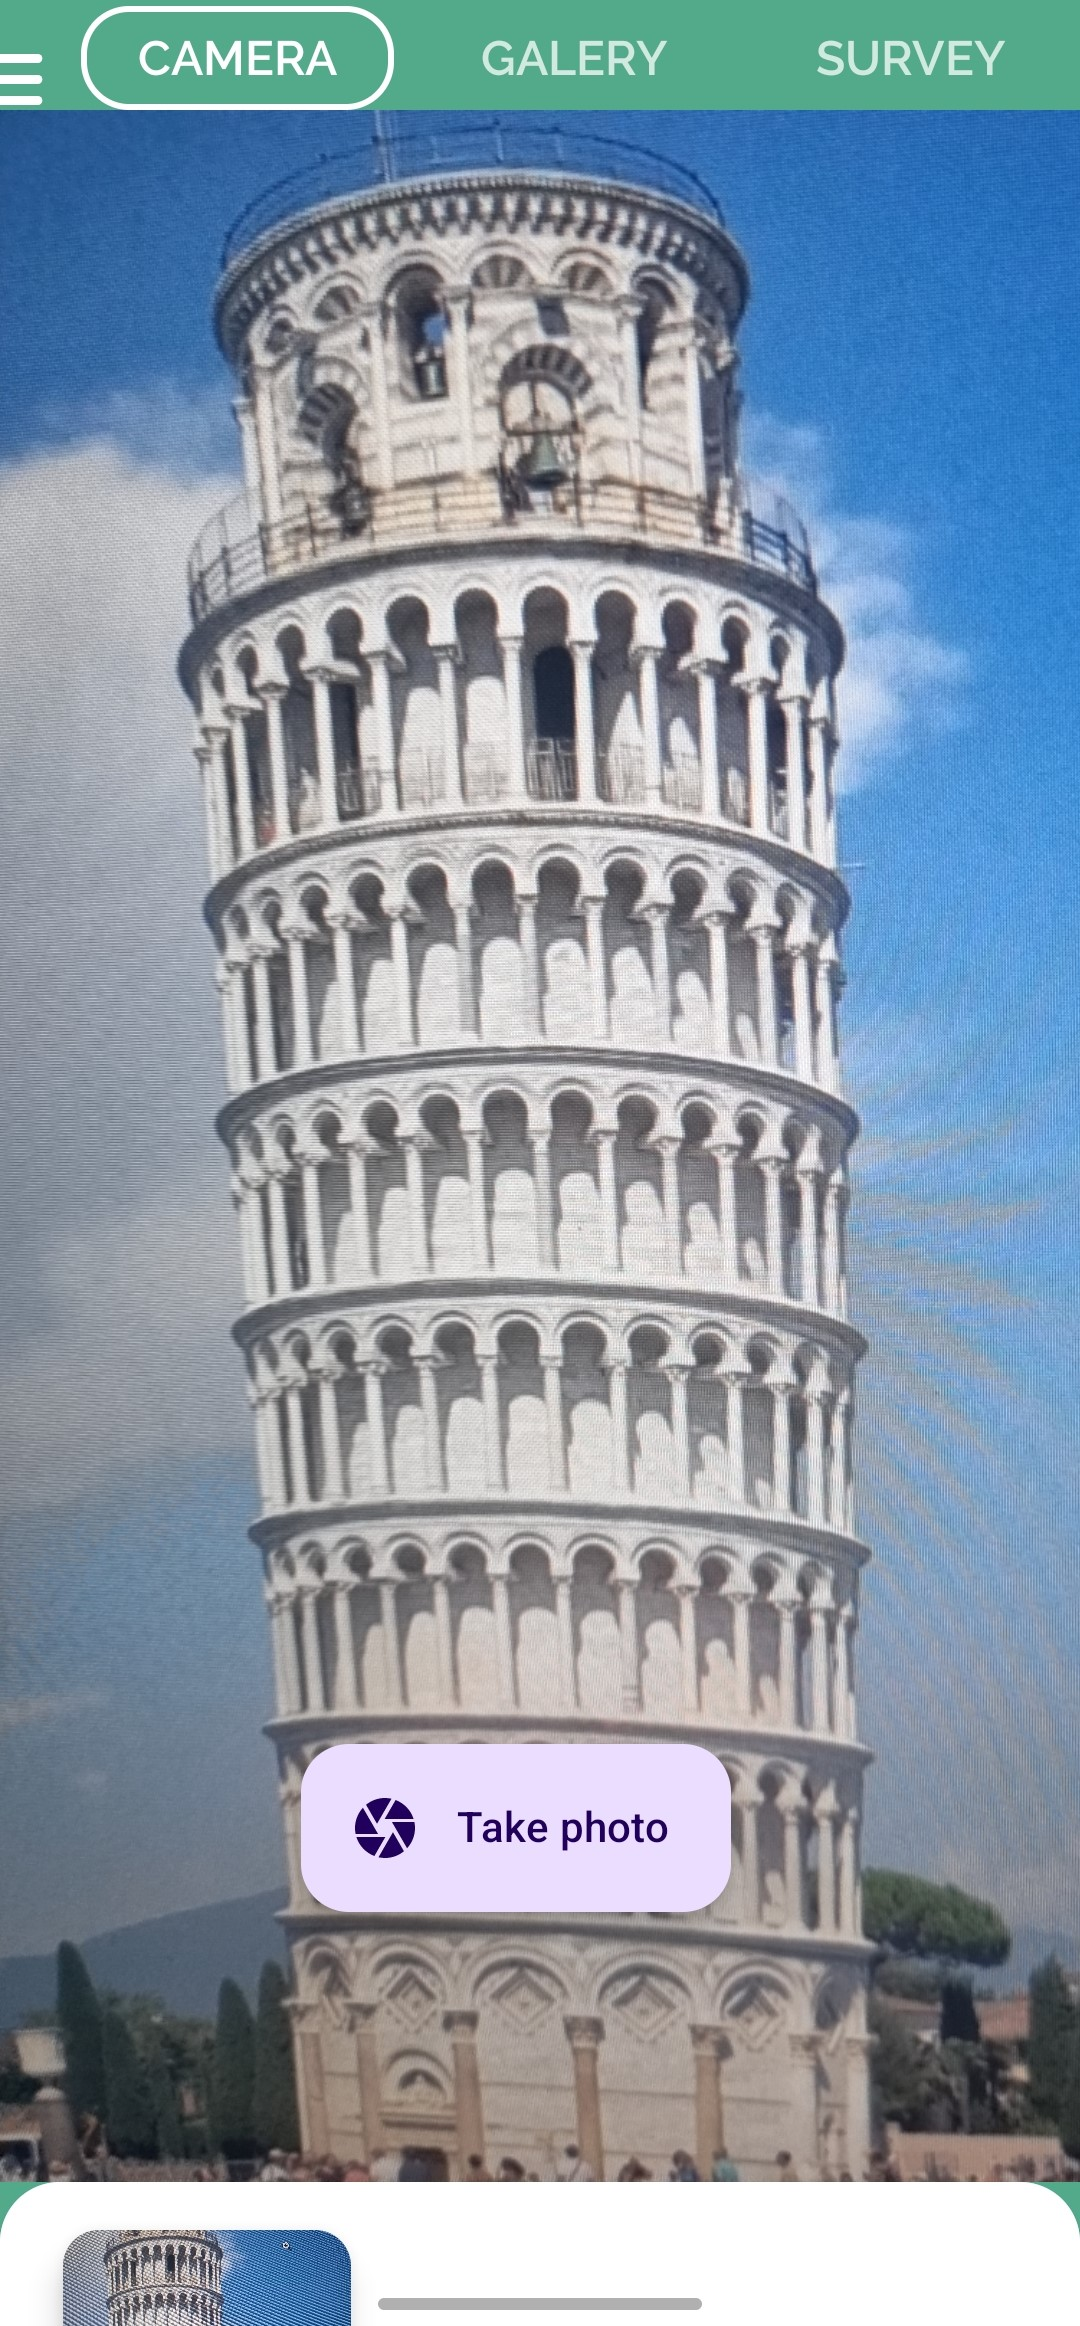
\includegraphics[width=0.5\textwidth]{camera.jpg}
    \captionsetup{justification=centering}
    \caption{Hier kan de gebruiker een foto nemen van de culturele erfgoed.}
    \label{fig:FrontEndCamera}
\end{figure}
\begin{figure}[h!]
    \centering
    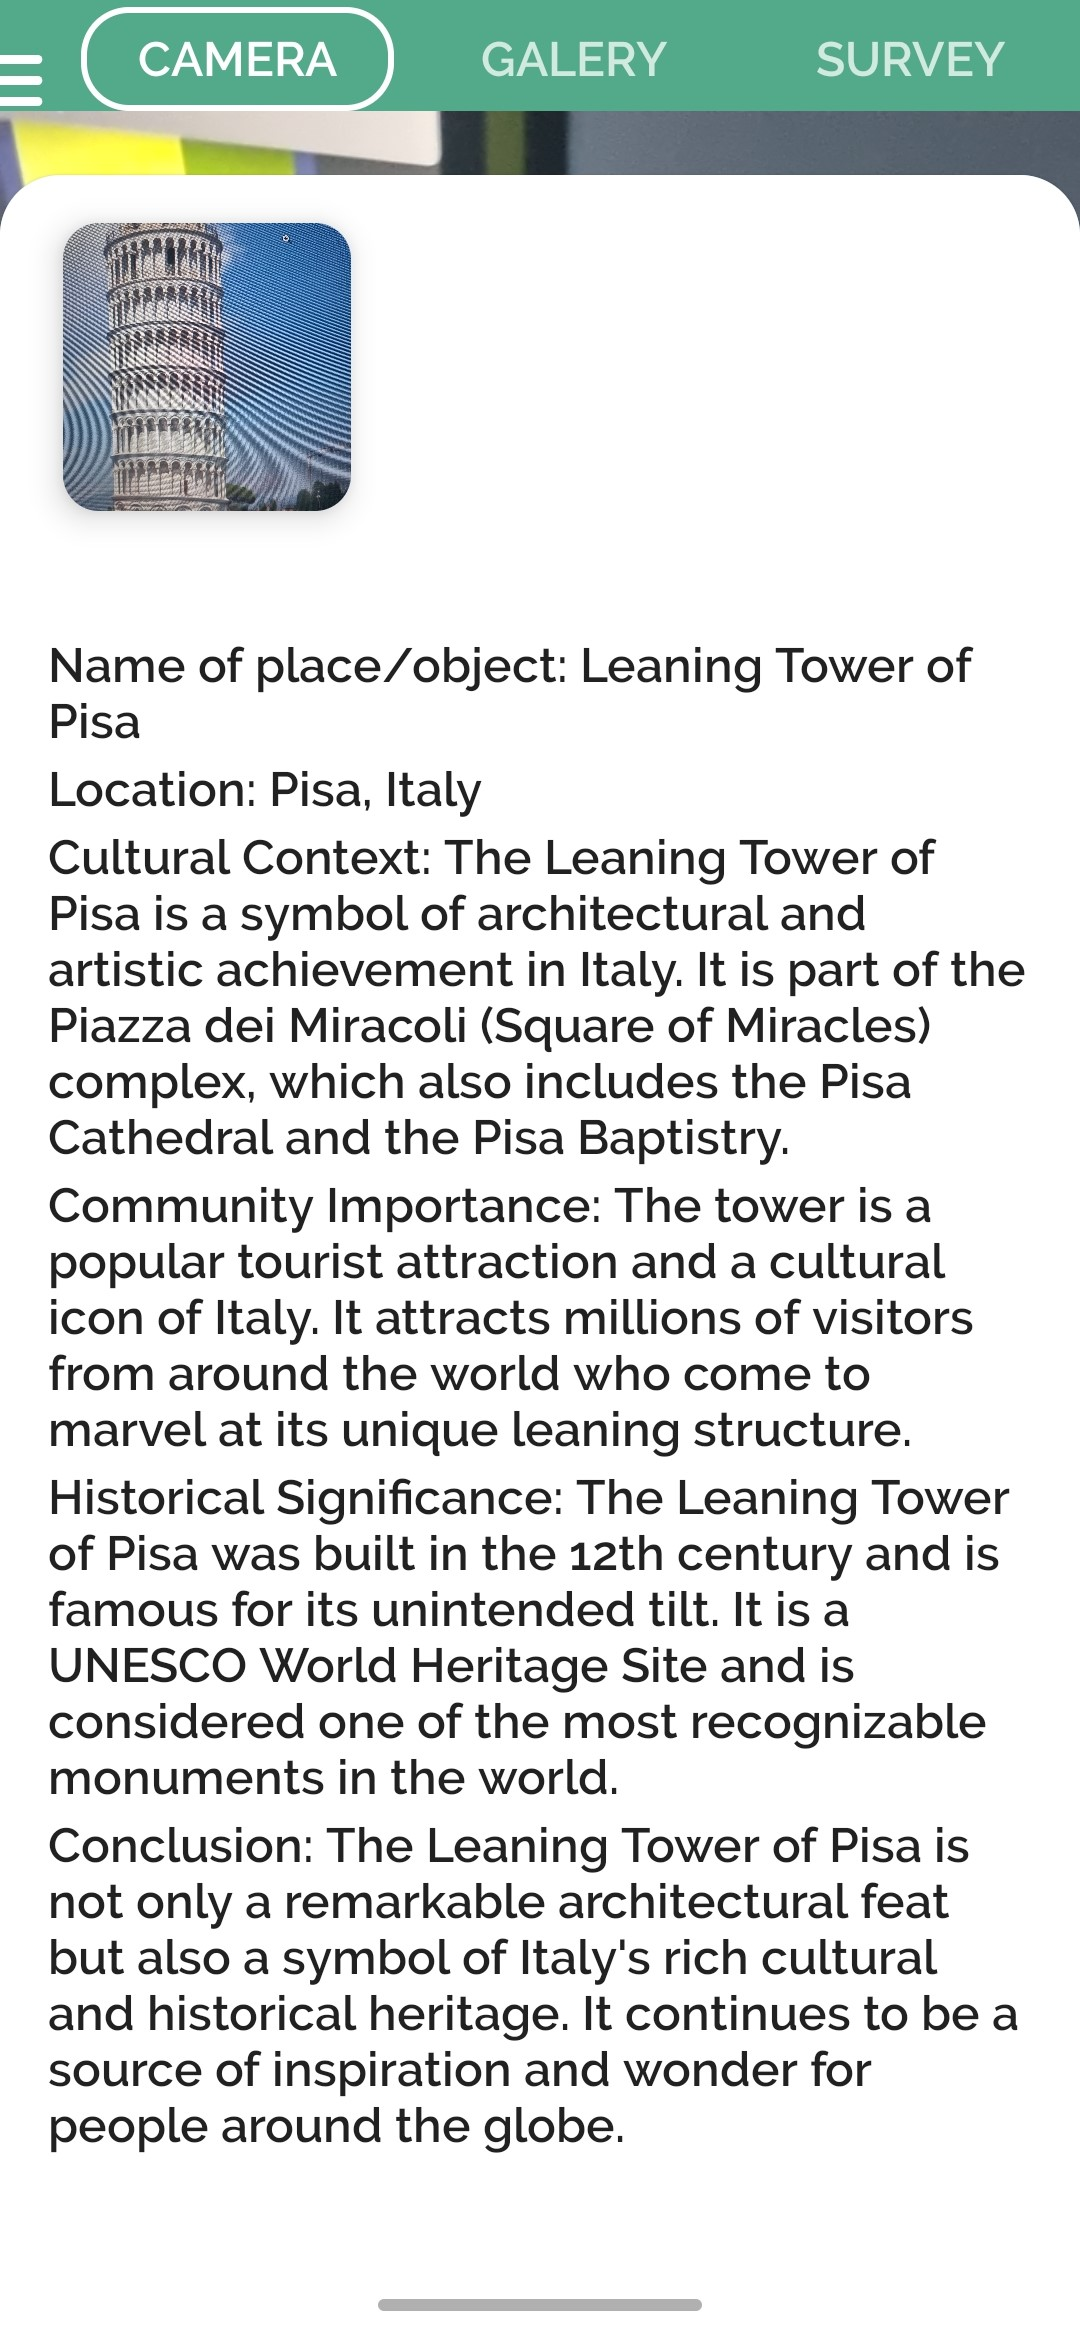
\includegraphics[width=0.5\textwidth]{details.jpg}
    \captionsetup{justification=centering}
    \caption{Hier wordt de door AI gegenereerde tekst weergegeven van het culturele erfgoed waarvoor een foto is genomen.}
    \label{fig:FrontEndCameraDetails}
\end{figure}
\pagebreak
\section{Java Backend}
De backend van het systeem is ontwikkeld in Java, gebruikmakend van het Spring Boot framework, dat efficiëntie en kracht biedt voor enterprise-level applicaties. Deze sectie beschrijft de ontwikkeling, functionaliteiten en belangrijkste technologieën die gebruikt zijn voor de Java-backend \autocite{VisionBackEnd}.

\begin{itemize}
    \item \textbf{API-ontwerp:} De backend fungeert als de centrale hub voor gegevensverwerking en is verantwoordelijk voor het ontvangen van afbeeldingen van de Android-applicatie, het communiceren met de Vision API en ChatGPT, en het opslaan van gegevens in de SQL-database. RESTful API's zijn geïmplementeerd met Spring Web, wat een gestandaardiseerde manier biedt voor het creëren van eindpunten en het behandelen van clientverzoeken.
    
    \item \textbf{Beeldvoorverwerking:} Voordat afbeeldingen worden doorgestuurd naar de Vision API, voert de backend cruciale voorverwerkingstaken uit zoals het resizen, comprimeren en eventueel het aanpassen van de belichting van de afbeeldingen om de nauwkeurigheid van de beeldanalyse te maximaliseren. Deze processen worden ondersteund door krachtige Java-bibliotheken zoals Java Advanced Imaging (JAI).
    
    \item \textbf{Beveiliging:} Veiligheid is een prioriteit in de ontwikkeling van de backend. Spring Security wordt gebruikt voor het authenticeren en autoriseren van gebruikers, het beveiligen van eindpunten, en het beschermen van gegevensoverdrachten met HTTPS. Bovendien zijn JWT-tokens geïmplementeerd voor een veilige, staatloze gebruikerssessiebeheer.
    
    \item \textbf{Databeheer:} Spring Data JPA wordt gebruikt voor het beheren van databasetransacties en het orkestreren van het data flow proces naar de SQL-database. Het maakt een efficiënte interactie met de database mogelijk via een abstractielaag die automatisch SQL-queries genereert uit repository methoden.
    
\end{itemize}


\pagebreak

\section{Vision API Integratie}
De integratie van Google's Vision API speelt een cruciale rol in de verwerking van afbeeldingen binnen het systeem. Deze sectie bespreekt de implementatie, het gebruik en de belangrijkste voordelen van de Vision API in het kader van dit project.

\begin{itemize}
    \item \textbf{Implementatie:} De Vision API wordt aangesproken via de Java-backend, waarbij gebruik wordt gemaakt van HTTP-verzoeken om afbeeldingen door te sturen en de analysegegevens te ontvangen. Deze integratie vereist nauwgezette configuratie van API-sleutels en verzoeksparameters om de functionaliteit en veiligheid te garanderen.
    
    \item \textbf{Beeldanalyse:} De API is in staat om complexe beelden te analyseren en een breed scala aan visuele gegevens te identificeren, waaronder objectherkenning, tekstextractie en gezichtsdetectie. Deze mogelijkheden zijn essentieel voor het systeem om relevante en nauwkeurige informatie te verstrekken over culturele en historische objecten.
    
    \item \textbf{Gegevensverwerking:} Na ontvangst van de analyse van de Vision API, worden de gegevens verwerkt door de backend. Dit omvat het filteren en formatteren van de data om deze geschikt te maken voor gebruik door ChatGPT voor contentgeneratie.
    
    \item \textbf{Voordelen en Uitdagingen:} Het gebruik van de Vision API biedt significante voordelen, zoals verbeterde nauwkeurigheid en snelheid van gegevensverwerking. Echter, er zijn ook uitdagingen zoals het beheersen van de kosten, het omgaan met de beperkingen van de API-quota, en het verzekeren van de privacy en veiligheid van de verwerkte gegevens.
\end{itemize}
\pagebreak
\subsection{Code}
Hier is een voorbeeld van de code die de Google Vision API gebruikt om webdetecties te vinden. Deze code stuurt een afbeelding naar de Vision API en verwerkt de resultaten van de webdetectie. De volledige documentatie is te vinden bij \autocite{googleVisionAPI}.

\begin{lstlisting}[caption={Voorbeeld van een Java-klasse die de Google Vision API gebruikt om webdetecties te vinden. Gebaseerd op de documentatie van \autocite{googleVisionAPI}},label={lst:googlevisioncode}]
    package org.example;
    import com.google.cloud.vision.v1.*;
    import com.google.cloud.vision.v1.Feature.Type;
    import com.google.protobuf.ByteString;
    import org.springframework.web.multipart.MultipartFile;
    import java.io.IOException;
    import java.util.ArrayList;
    import java.util.List;
    
    public class DetectWebDetectionsImage {
        public static String detectWebDetections(MultipartFile file) throws IOException {
            List<AnnotateImageRequest> requests = new ArrayList<>();
            StringBuilder results = new StringBuilder();
            ByteString imgBytes = ByteString.copyFrom(file.getBytes());
            Image img = Image.newBuilder().setContent(imgBytes).build();
            Feature feat = Feature.newBuilder().setType(Type.WEB_DETECTION).build();
            AnnotateImageRequest request =
            AnnotateImageRequest.newBuilder().addFeatures(feat).setImage(img).build();
            requests.add(request);
            
            try (ImageAnnotatorClient client = ImageAnnotatorClient.create()) {
                BatchAnnotateImagesResponse response = client.batchAnnotateImages(requests);
                List<AnnotateImageResponse> responses = response.getResponsesList();
                for (AnnotateImageResponse res : responses) {
                    if (res.hasError()) {
                        System.out.format("Error: %s%n", res.getError().getMessage());
                        return "Error: " + res.getError().getMessage();
                    }
                    WebDetection annotation = res.getWebDetection();
                    results.append("Entity:Id:Score\n==============\n");
                    annotation.getWebEntitiesList().forEach(entity ->
                    results.append(entity.getDescription()).append(" : ")
                    .append(entity.getEntityId()).append(" : ")
                    .append(entity.getScore()).append("\n"));
                    annotation.getBestGuessLabelsList().forEach(label ->
                    results.append("\nBest guess label: ").append(label.getLabel()).append("\n"));
                    results.append("\nPages with matching images: Score\n==\n");
                    annotation.getPagesWithMatchingImagesList().forEach(page ->
                    results.append(page.getUrl()).append(" : ").append(page.getScore()).append("\n"));
                    results.append("\nPages with partially matching images: Score\n==\n");
                    annotation.getPartialMatchingImagesList().forEach(image ->
                    results.append(image.getUrl()).append(" : ").append(image.getScore()).append("\n"));
                    results.append("\nPages with fully matching images: Score\n==\n");
                    annotation.getFullMatchingImagesList().forEach(image ->
                    results.append(image.getUrl()).append(" : ").append(image.getScore()).append("\n"));
                    results.append("\nPages with visually similar images: Score\n==\n");
                    annotation.getVisuallySimilarImagesList().forEach(image ->
                    results.append(image.getUrl()).append(" : ").append(image.getScore()).append("\n"));
                }
                return results.toString();
            }
        }
    }    
\end{lstlisting}

\section{Output}

Hier is een voorbeeld van een culturele erfgoedsite, het Colosseum in Rome:

\begin{figure}[h!]
    \centering
    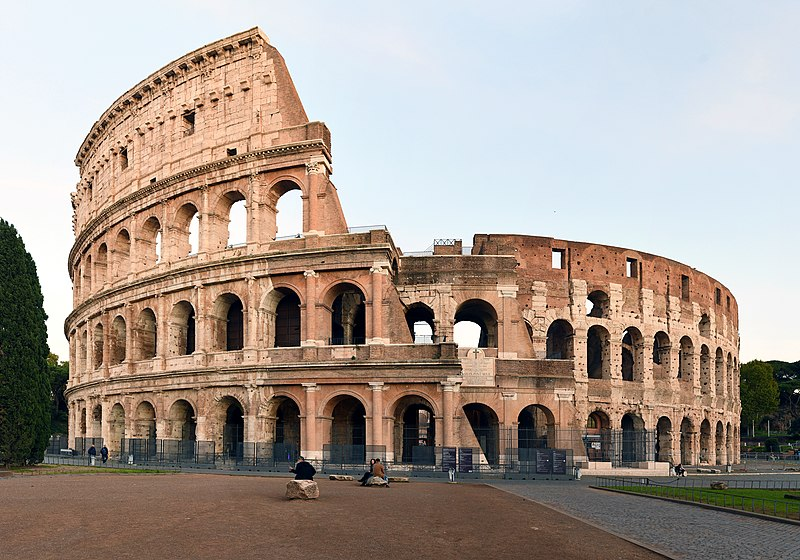
\includegraphics[width=\textwidth]{colosseum.jpg}
    \caption{Het Colosseum in Rome \autocite{wikimediaColosseum}.}
    \label{fig:colosseum}
\end{figure}
\pagebreak

Hieronder zien we de output die verkregen wordt als we de afbeelding in \autoref{fig:colosseum} meegeven aan de Vision API met de code in \autoref{lst:googlevisioncode}.

\begin{lstlisting}[caption={Output vision api},label={lst:outputvisionapi}]
    Entity:Id:Score
    ==============
    Colosseum : /m/0d5qx : 1.7518381
    Ancient Rome : /m/02l341 : 1.1704171
    Roman Forum : /m/0n16t : 1.0100476
    Amphitheater : /m/0f48p : 0.7254882
    Palatine Hill : /m/015376 : 0.679173
    Ancient Roman architecture : /m/0dvg9 : 0.6050097
    Roman amphitheatre : /m/0h1fm4h : 0.5354
    Monument : /m/02ljgl : 0.4356
    : /t/2cs7w02wlkht2 : 0.3742
    Cavea : /m/02drdx : 0.3601
    
    Best guess label: colosseum rome
    
    Pages with matching images: Score
    ==
    https://en.wikipedia.org/wiki/Colosseum : 0.0
    https://www.quora.com/Have-you-been-to-the-Rome-Colosseum-What-did-you-think-when-you-first-saw-it-And-how-did-it-make-you-feel-being-there : 0.0
    https://www.institutodecegosdabahia.org.br/colosseum-ancient-rome-tour-with-gladiator-s-gate-small-dd-EonkR2CW : 0.0
    https://www.quora.com/I-recently-visited-the-Colosseum-and-felt-completely-insignificant-in-its-presence-What-are-other-sites-that-have-made-people-feel-that-way : 0.0
    https://www.italyrometour.com/what-happened-to-the-marbles-that-decorated-the-colosseum/ : 0.0
    https://www.institutodecegosdabahia.org.br/immerse-yourself-in-colosseum-rome-explore-the-iconic-landmark-dd-RWgARpiB : 0.0
    https://aleteia.org/2022/05/04/the-secret-chapel-inside-romes-colosseum/ : 0.0
    https://www.reddit.com/r/todayilearned/comments/18llju0/til_we_dont_know_what_the_romans_called_the/ : 0.0
    https://www.fnh.edu.br/?y=sunrise-at-colosseum-rome-italy-stock-photo-download-image-11-pp-zmZljnuk : 0.0
    https://gbu-hamovniki.ru/announcement/?k=the-colosseum-in-rome-all-things-you-should-know-uu-XR6y1yca : 0.0
    
    Pages with partially matching images: Score
    ==
    https://pbs.twimg.com/card_img/1785266653099438080/bmKNDfRd?format=jpg&name=900x900 : 0.0
    https://media.licdn.com/dms/image/sync/D4D27AQG4QGY9Szh96Q/articleshare-shrink_800/0/1712043042683?e=2147483647&v=beta&t=ezihVY30Lw0-I9UBdYp3_UDIi73UDotxKHSyEFLobv8 : 0.0
    https://i0.wp.com/www.re-thinkingthefuture.com/wp-content/uploads/2022/03/A6454-Keypoints-to-remember-while-understand-roles-of-proportion-in-aesthetics-Image-2.jpg?w=999 : 0.0
    https://lookaside.fbsbx.com/lookaside/crawler/media/?media_id=10223761936025640 : 0.0
    https://howtorhino.com/wp-content/uploads/2023/11/Ancient-Greek-Architecture-22.jpg : 0.0
    https://s2.abcstatics.com/abc/www/multimedia/sevilla/2024/05/08/coliseo-de-roma-RVk0A59wxmwbLirx6Rzm78K-1200x840@diario_abc.jpg : 0.0
    https://i0.wp.com/arteyalgomas.com/wp-content/uploads/2023/03/Coliseo.jpg?resize=840%2C588&quality=89&ssl=1 : 0.0
    https://lookaside.fbsbx.com/lookaside/crawler/media/?media_id=227847066251442 : 0.0
    https://images.techinsider.ru/upload/img_cache/36c/36ccb6f688aa3ab359b22f8084f4cd41_cropped_510x357.jpg : 0.0
    https://www.libremedia.ca/wp-content/uploads/2024/01/1704788233_935_le-classement-des-villes-et-sites-culturels-les-plus-visites.jpeg : 0.0
    
    Pages with fully matching images: Score
    ==
    https://static.android.com.pl/uploads/2023/11/starozytny_rzym_koloseum-scaled.jpg : 0.0
    https://image.spletnik.ru/resize/fit=contain,gravity=0.5x0.5,format=auto,width=1011,height=700,dpr=2/https://image.spletnik.ru/image/2023/06/30/-xw_/original.webp : 0.0
    https://image.spletnik.ru/image/2023/06/30/-xw_/original.webp : 0.0
    http://pic.yupoo.com/fotomag/82123b11/26c91368.jpg : 0.0
    https://upload3.inven.co.kr/upload/2022/07/07/bbs/i13854160493.jpg : 0.0
    https://cdn4.dogonews.com/images/7579050a-0960-470c-bd8c-dae841129103/1920px-colosseo_2020.jpeg : 0.0
    https://assets-global.website-files.com/61d563faa9a56900d65ee25c/62971926a4f2df0997fa5d10_Foto%202.jpg : 0.0
    http://www.apartamento203.com.br/wp-content/uploads/2023/04/Colosseo_2020.jpg : 0.0
    https://lookaside.fbsbx.com/lookaside/crawler/media/?media_id=361667810214259 : 0.0
    https://www.sapiens.cat/uploads/s1/13/88/18/1/roma.webp : 0.0
    
    Pages with visually similar images: Score
    ==
    https://upload.wikimedia.org/wikipedia/commons/thumb/d/de/Colosseo_2020.jpg/1200px-Colosseo_2020.jpg : 0.0
    https://colosseo.it/sito/wp-content/uploads/2018/11/colosseo_esterno.jpg : 0.0
    https://www.pic.int/Portals/5/images/Rome.jpg : 0.0
    https://www.waseda.jp/top/assets/uploads/2024/01/waseda_20240122_img3-360x270.jpg : 0.0
    https://media.beniculturali.it/mibac/files/boards/be78e33bc8ca0c99bff70aa174035096/Luoghi/Parco%20archeologico%20del%20Colosseo%20-%20Colosseo.%20Anfiteatro%20Flavio.jpg : 0.0
    https://cdn.britannica.com/36/162636-131-E4AA93A0/Colosseum-Rome-Italy.jpg : 0.0
    http://pop.h-cdn.co/assets/17/40/3200x1600/landscape-1507135566-colosseum-exterior-inner-and-outer-wall-avl.jpg : 0.0
    https://cdn.getyourguide.com/img/tour/f9964a688f184da5.jpeg/70.jpg : 0.0
    https://st3.idealista.it/news/archivie/styles/highlighted_sm/public/2024-05/images/rome-3550739_1920.jpg?VersionId=rk8PKjYQDOV8smAywUVsKP_M1zZ_9Aux&itok=qUm4fyYX : 0.0
    https://www.odu.edu/sites/default/files/styles/homepage_hero_image/public/images/2022-11/AdobeStock_119146497.jpeg?h=901541b5 : 0.0
\end{lstlisting}

\section{ChatGPT 3.5 Integratie}
De integratie van OpenAI's ChatGPT 3.5 is van cruciaal belang voor het omzetten van visuele data geanalyseerd door de Vision API in gedetailleerde tekstuele beschrijvingen die cultureel en historisch inzicht bieden. Deze integratie maakt gebruik van geavanceerde natuurlijke taalverwerking om informatieve content te genereren die de gebruiker helpt de betekenis en het belang van de bezienswaardigheden te begrijpen.

\subsection{Gegevensverwerking en -integratie}
Na de verwerking van afbeeldingen door de Vision API, waarbij zowel webdetectie als objectherkenning worden toegepast, worden deze data samengevoegd in een gestructureerde output die de basis vormt voor tekstgeneratie. 

\begin{itemize}
    \item \textbf{Data Samenvoeging:} De output van de Vision API, die bestaat uit kenmerken zoals objectherkenning en webdetectiegegevens, wordt gecombineerd tot een enkele samenvattende beschrijving van de afbeelding.
    
    \item \textbf{Prompt Opbouw:} Deze samenvatting wordt dan gebruikt als input voor ChatGPT 3.5 met een specifieke prompt: \texttt "based on this data give information about Name of place/object, Location and Cultural Context, Community Importance, Historical Significance, Conclusion". Deze prompt vraagt ChatGPT 3.5 om uitgebreide informatie te genereren over de naam van de plaats of het object, locatie, culturele context, belang voor de gemeenschap, historische significantie, en een afsluitende conclusie.
\end{itemize}

\subsection{Content Generatie door ChatGPT 3.5}
Op basis van de geformuleerde prompt, genereert ChatGPT 3.5 diepgaande, relevante tekstuele content die rijk is aan culturele en historische informatie.

\begin{itemize}
    \item \textbf{Tekstuele Output:} De gegenereerde teksten bieden uitgebreide informatie die essentieel is voor educatieve en culturele interpretatie door de eindgebruiker.
    \item \textbf{Dynamische Content Aanpassing:} Doorlopende feedback van gebruikers wordt geanalyseerd om de nauwkeurigheid en relevantie van de gegenereerde informatie continu te verbeteren.
\end{itemize}

\subsection{Voordelen en Uitdagingen}
De integratie van ChatGPT 3.5 verrijkt de applicatie aanzienlijk door diepgaande en contextueel relevante beschrijvingen te bieden, maar brengt ook uitdagingen met zich mee zoals de afhankelijkheid van de nauwkeurigheid van de Vision API data en de beheersing van operationele kosten.

\subsection{Implementatievoorbeeld}
Hier krijgen we aan de hand van de input van de Vision API in \autoref{lst:outputvisionapi} deze data van ChatGPT 3.5:

\begin{quote}
“Naam van de Plaats/Het Object
Colosseum (ook bekend als het Flavische Amfitheater).

Locatie
Gelegen in het centrum van Rome, Italië, is het Colosseum een onmiskenbaar herkenningspunt in het historische landschap van de stad, in de buurt van andere belangrijke ruïnes zoals het Forum Romanum en de Palatijn.

Culturele Context
Het Colosseum is een essentieel symbool van de Romeinse ingenieurskunst en cultuur uit de oudheid. Het werd voornamelijk gebruikt voor gladiatorengevechten en openbare spektakels zoals nagespeelde zeeslagen, dierengevechten, executies, reconstructies van beroemde veldslagen en drama’s gebaseerd op klassieke mythologie. Dit amfitheater kon tussen de 50.000 en 80.000 toeschouwers houden, wat de architectonische en technische kunde van de oude Romeinen toont.

Belang voor de Gemeenschap
Het Colosseum blijft een cruciaal herkenningspunt in Rome, niet alleen als een belangrijke toeristische attractie die jaarlijks miljoenen bezoekers trekt, maar ook als een symbool van de rijke historische en culturele erfgoed van Rome. Het staat als een bewijs van de vindingrijkheid van de oude Romeinse architectuur en heeft invloed gehad op het ontwerp van moderne sportstadions.

Historische Betekenis
Gebouwd onder de Flavische keizers tussen 72 en 80 na Christus, weerspiegelt het Colosseum de overgang van de Republiek naar het Keizerrijk in de Romeinse geschiedenis. Het heeft talrijke aardbevingen en diefstallen van stenen doorstaan en blijft grotendeels intact, wat inzicht biedt in de levensstijl, sociale structuur en bestuur van het oude Rome. Het was niet alleen een locatie voor sport en entertainment, maar ook een demonstratie van de macht van het keizerlijke Rome en de sociale stratificatie die heerste in de Romeinse samenleving.

Conclusie
Het Colosseum is niet alleen een architectonisch hoogstandje; het is een cultureel icoon dat de tand des tijds heeft doorstaan, een venster biedend op de oude beschaving van Rome en blijft de esthetiek en functionaliteit van de moderne architectuur beïnvloeden. Het omvat de grandeur van het oude Rome en blijft een centraal onderdeel van de identiteit van Rome en een cruciale locatie voor het begrijpen van de menselijke geschiedenis en cultuur.”
\end{quote}

